\documentclass{article}

\usepackage{tikz}
\usepackage{tkz-graph}
\usepackage{tkz-berge}

\begin{document}

Este es un ejemplo:
\begin{center}
  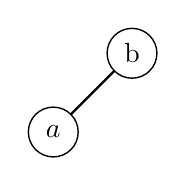
\begin{tikzpicture}
    \Vertex[x=0,y=0,Math]{a}
    \Vertex[x=1,y=1]{b}
    \Edge(a)(b)
  \end{tikzpicture}
\end{center}

\begin{center}
  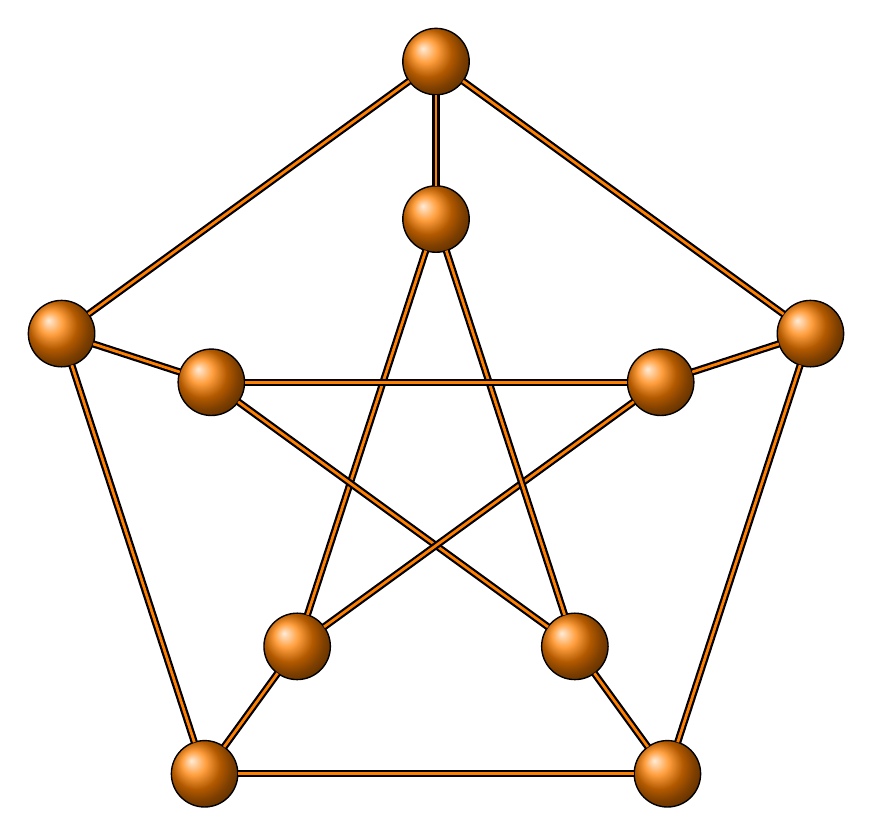
\begin{tikzpicture}
    \GraphInit[vstyle=Shade]
    \GraphInit[vstyle=Art]
    \SetVertexNoLabel
    \grPetersen[Math,rotation=90,RA=5,RB=3]
  \end{tikzpicture}
\end{center}

\begin{center}
  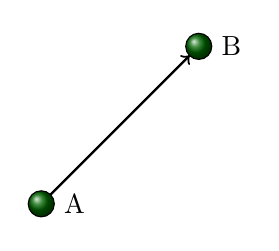
\begin{tikzpicture}
    \GraphInit[vstyle=Classic]
    \tikzset{VertexStyle/.style = {%
        shape= circle,
        shading= ball,
        ball color= green!40!black,%
        minimum size = 2pt,draw}}
    \Vertex[x=0,y=0]{A}
    \Vertex[x=2,y=2]{B}
    \Edge[style={->}](A)(B)
    \Edge(A)(B)
    %\Vertex{A}\EA[unit=10]
  \end{tikzpicture}
\end{center}

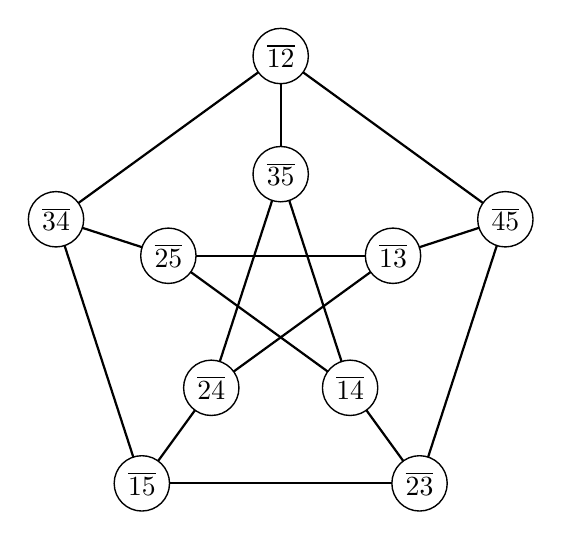
\begin{tikzpicture}[rotate=90,scale=1]
  \newcommand{\aset}[2]{$\{#1,#2\}$}
  \GraphInit[vstyle=Classic]
  %\tikzset{VertexStyle/.style={draw,circle}}
  \SetVertexNoLabel
  \SetVertexMath
  \SetUpVertex[MinSize=20pt]
  \grPetersen[RA=3,RB=1.5]
  \AssignVertexLabel{a}{\textsl{$\overline{12}$},\textsl{$\overline{34}$},\textsl{$\overline{15}$},\textsl{$\overline{23}$},\textsl{$\overline{45}$}}
  \AssignVertexLabel{b}{\textsl{$\overline{35}$},\textsl{$\overline{25}$},\textsl{$\overline{24}$},\textsl{$\overline{14}$},\textsl{$\overline{13}$}}
\end{tikzpicture}

\end{document}
